\section{Explaining the Phenomena of Negative Transfer in Multi-Task Learning}\label{sec_insight}

Based on the key lemma, we provide rigorous explanations to the phenomena of negative transfer in multi-task learning.
We study three components, including task model, data size and covariate shift.
For each component, we show how negative transfer occurs using a simplified isotropic model.
Then, we describe the algorithmic consequence of the theory.

\subsection{Task Model}\label{sec_similarity}

It is well-known since the seminal work of Caruana \cite{C97} that how well multi-task learning performs depends on task relatedness.
As a warmup, we first describe an example that rigorously formalizes the connection using our setup.

\textit{The isotropic model.}
	Consider two tasks with isotropic covariances $\Sigma_1 = \Sigma_2 = \id$.
	Recall that each task has data size $n_i = \rho_i \cdot p$, for $i = 1, 2$.
	And $X_1\in\real^{n_1\times p}, X_2\in\real^{n_2\times p}$ denotes the covariates of the two tasks, respectively.
	We assume that for the target task, $\beta_2$ has i.i.d. entries with mean zero and variance $\kappa^2$.
	For the source task, $\beta_1 $ equals $\beta_2$ plus i.i.d. entries with mean $0$ and variance $d^2$.
	The labels are given by $Y_i = X_i\beta_i + \varepsilon_i$, where $\e_i$ consists of i.i.d. entries with mean zero and variance $\sigma_i^2$, for $i=1,2$.
	\footnote{For simplicity, we assume that all the random variables have subexponential decay, while keeping in mind that our results can be applied under weaker moments assumptions as shown in the supplementary material.}

We measure model dissimilarity as $\norm{\beta_1 - \beta_2}^2$, which is the distance between source and target in the isotropic model.
We derive a sharp threshold when positive transfer transitions to negative transfer, as model dissimilarity increases.
%Based on Theorem \ref{thm_model_shift}, we derive the transition threshold in the following proposition.
Define the following functions
\begin{align*}
	\Psi(\beta_1, \beta_2) = {\ex{\bignorm{\beta_1 - \beta_2}^2}} / {\sigma^2},  \quad \Phi(\rho_1, \rho_2) = \frac{(\rho_1 + \rho_2 - 1)^2}{\rho_1 (\rho_1 + \rho_2) (\rho_2 - 1)}.
\end{align*}
Let $\gamma_{-} = (1-\oo(1))\cdot(1 - \rho_1^{-1/2})^4$ and $\gamma_{+} = (1+\oo(1))\cdot(1 + \rho_1^{-1/2})^4$.
Concretely, if $\rho_1 > 40$, then $\gamma_{-} < 2$ and $\gamma_{+} > 1/2$.

\begin{proposition}[Model dissimilarity]\label{prop_dist_transition}
	In the isotropic model, suppose that $\rho_1 > 1$ and $\sigma_1 = \sigma_2 = \sigma$.
	Then we have that
	%Whether $\te(\hat{\beta}_t^{\MTL})$ is lower than $\te(\hat{\beta}_t^{\STL})$ is determined by the ratio between $\Psi(\beta_1, \beta_2)$ and $\Phi(\rho_1, \rho_2)$:
	\squishlist
		\item If $\Psi(\beta_1, \beta_2) < \gamma_{-} \cdot \Phi(\rho_1, \rho_2)$, then whp we have that $\te(\hat{\beta}_t^{\MTL}) < \te(\hat{\beta}_t^{\STL})$.
		\item If $\Psi(\beta_1, \beta_2) \ge \gamma_{+} \cdot \Phi(\rho_1, \rho_2)$, then whp we have that $\te(\hat{\beta}_t^{\MTL}) \ge \te(\hat{\beta}_t^{\STL})$.
	\squishend
\end{proposition}

Proposition \ref{prop_dist_transition} simplifies Theorem \ref{thm_main_informal} in the isotropic model, allowing for a more explicit statement of the bias-variance tradeoff.
\todo{} We illustrate the example with a simulation.
We consider a setting where $p = 200$, $n_1 = 90p$, $n_2 = 30p$.
We fix the target task and vary the source task, in particular the parameter $d$ which determines $\norm{\beta_1 - \beta_2}$.
Figure \ref{fig_model_shift} shows the result.
We observe that Proposition \ref{prop_dist_transition} explains most of the observations in Figure \ref{fig_model_shift}.


The proof of Proposition \ref{prop_dist_transition} involves two parts.
First, in equation \eqref{eq_te_var}, the positive variance reduction effect scales with $n_1 = \rho_1 p$, the number of source task data points.
Second, we show that the negative effect of model-shift bias scales with $pd^2$, which is the expectation of $\norm{\beta_1 - \beta_2}^2$.
The proof, which is based on Theorem \ref{thm_main_informal}, can be found in Appendix \ref{app_proof_31}. %, which is based on our main result described later in Theorem \ref{thm_model_shift}.

\begin{figure}
	\begin{subfigure}[b]{0.32\textwidth}
		\centering
		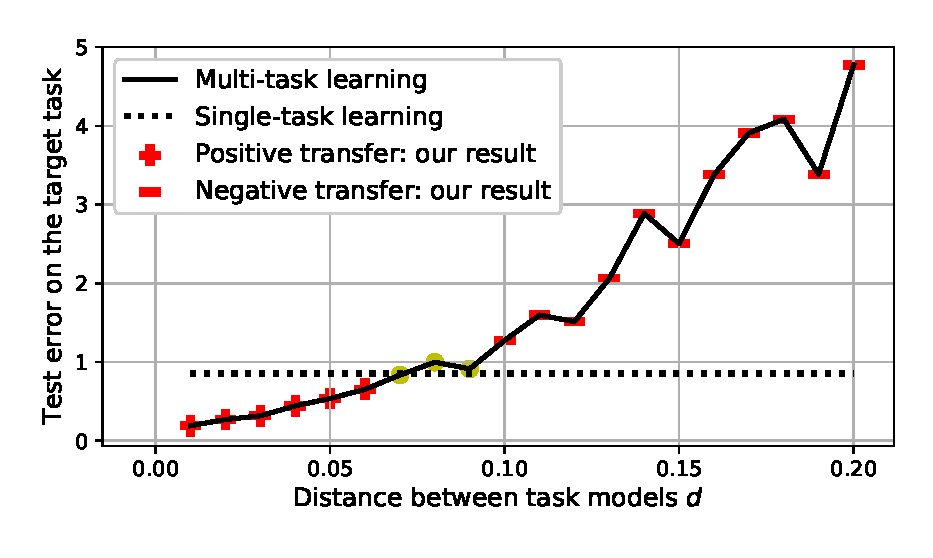
\includegraphics[width=0.98\textwidth]{figures/model_shift_phase_transition.eps}
		\caption{Task model}
		\label{fig_model_shift}
	\end{subfigure}\hfill
	\begin{subfigure}[b]{0.32\textwidth}
		\centering
		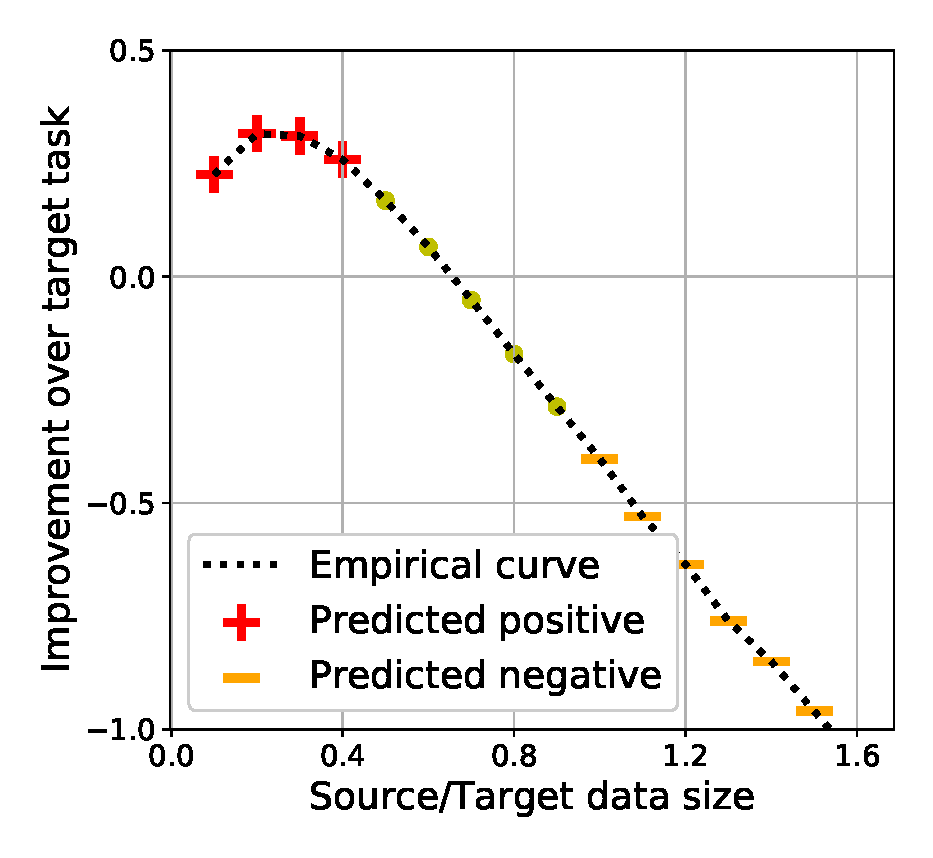
\includegraphics[width=0.98\textwidth]{figures/datapoints_phase_transition.eps}
		\caption{Data size}
	\end{subfigure}\hfill
	\begin{subfigure}[b]{0.32\textwidth}
		\centering
		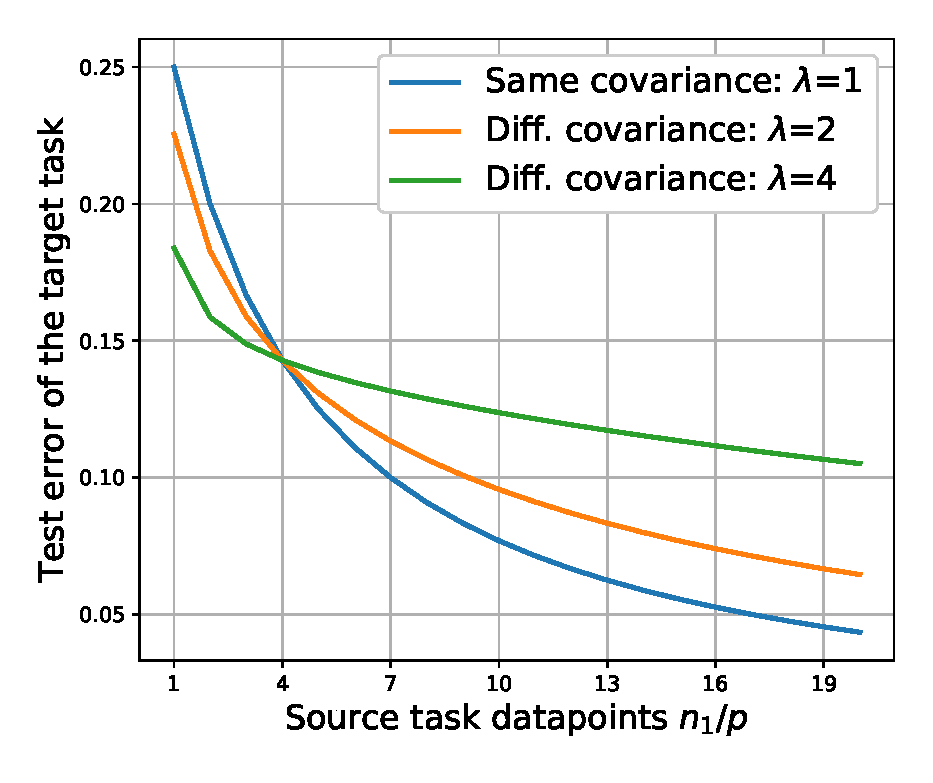
\includegraphics[width=0.98\textwidth]{figures/complementary.eps}
		\caption{Covariate shift}
		\label{fig_covariate}
	\end{subfigure}
	\caption{Three contributing causes of negative transfer:
	(a) As model dissimilarity increases, we observe a transition from positive to negative transfer  (Proposition \ref{prop_dist_transition}).
	(b) As source task data size increases, we observe a transition positive to negative transfer (Proposition \ref{prop_data_size}).
	(c) As covariate shift becomes more severe (measured by increasing $\lambda$), test performance gets worse (Proposition \ref{prop_covariate}).}
	\label{fig_model_shift_phasetrans}
\end{figure}

\textbf{Algorithmic consequence.}
We further show that multi-task learning is particular powerful when the labeled data of the source task is less noisy compared to the target task.
Consider a more general setting of Proposition \ref{prop_dist_transition} where the noise level $\sigma_1$ of task $1$ differs from the noise level $\sigma_2$ of task $2$.
If $\sigma_1$ is too large, then the source task provides a negative transfer to the target.
If $\sigma_1$ is small, then the transfer may be positive.
Proposition \ref{prop_var_transition} formalizes the intuition.

Based on the result, we propose a simple metric to determine whether multi-task learning performs better than single-task learning.
The metric is as follows.
First, we train 2 single-task models on 2 separate tasks.
We take the prediction accuracy of the two tasks.
Let $\tau$ be a fixed threshold.
If the accuracy of the source task is higher than the accuracy of the target task by $\tau$, then we predict positive transfer.
On the other hand, if the accuracy of the source task is lower than the accuracy of the target task by $\tau$, then we predict negative transfer.

\subsection{Data Size}
In classical Rademacher or VC based theory of multi-task learning, the generalization bounds are usually presented for settings where the data sizes are equal for all tasks \cite{B00,M06,MPR16}.
More generally, such results are still applicable when all task data are being added simultaneously.
On the other hand, for many applications of multi-task learning, the data sources are usually heterogeneous.
For such settings, we have observed that adding more labeled data from one task does not always help.
%On the other hand, we have observed that adding more labeled data does not always improve performance in multi-task learning.
Using the isotropic model, we consider what happens if we vary the source task data size.

\begin{proposition}[Unnecessary source data]\label{prop_data_size}
	In the isotropic model, assume that $\rho_1 > 40$ and $\rho_2 > 150$ are fixed constants, $\Psi(\beta_1, \beta_2) > 2/(\rho_2 - 1)$.
	We have that
	\squishlist
		\item If $\rho_1 < \frac{\rho_2-2}{\gamma_+ \cdot \Psi(\beta_1, \beta_2) (\rho_2 - 1) - 1}$, then w.h.p. $\te(\hat{\beta}_t^{\MTL}) < \te(\hat{\beta}_t^{\STL})$.
		\item If $\rho_1 > \frac{\rho_2-2}{\gamma_- \cdot \Psi(\beta_1, \beta_2) (\rho_2 - 3) - 1}$, then w.h.p. $\te(\hat{\beta}_t^{\MTL}) > \te(\hat{\beta}_t^{\STL})$.
	\squishend
\end{proposition}
Proposition \ref{prop_data_size} shows that as the source data size increases, we observe a transition from positive to negative transfer.
The proof of Proposition \ref{prop_data_size} is similar to Proposition \ref{prop_dist_transition}, and can be found in Appendix \ref{app_proof_31}.


We use our tools to explain a key result of taskonomy \cite{ZSSGM18}, which shows that by learning from multiple related tasks, one can reduce the amount of labeled data from each task.
This is formalized as follows.

Given several tasks, let the data efficiency ratio be the largest factor $x$ such that the total number of labeled datapoints needed for solving all tasks can be reduced by $x$ while keeping the same performance compared to STL.
%More precisely, suppose we have $n_i$ datapoints for each task, for $i= 1, 2$.
For $i = 1, 2$, let $\hat{\beta}_i^{\MTL}(x)$ denote the estimator trained using only $x \cdot n_i$ datapoints from every task.
The data efficiency ratio is defined as
\[ \argmin_{x\in(0, 1)} ~~
		\te_1(\hat{\beta}_1^{\MTL}(x)) + \te_2(\hat{\beta}_2^{\MTL}(x))
		\le \te_1(\hat{\beta}_1^{\STL}) + \te_2(\hat{\beta}_2^{\STL}). \]
We quantify the data efficiency ratio of the isotropic model as follows.

\begin{proposition}[Labeled data efficiency]\label{prop_data_efficiency}
	In the isotropic model, assume that $\rho_1,\rho_2 > 10$ and $\Psi(\beta_1, \beta_2) < \frac{2}{\rho_1} + \frac{2}{\rho_2}$.
	Then the data efficiency ratio is at least \[ \frac{1}{\rho_1 + \rho_2}\cdot \bigbrace{1 + \frac{1}{\rho_1^{-1} + \rho_2^{-1} - 5\Psi(\beta_1, \beta_2)}}. \]
\end{proposition}
The proof of Proposition \ref{prop_data_efficiency} can be found in Appendix \ref{app_proof_data}.

\textbf{Algorithmic consequence.} An interesting consequence of Proposition \ref{prop_data_size} is that the $L(\hat{\beta}_t^{\MTL})$ is not monotone in $\rho$.
Instead, from the analysis, we observe that $L(\hat{\beta}_t^{\MTL})$ is quadratic.
Based on this insight, we propose an incremental optimization schedule to improve MTL training efficiency.
Algorithm \ref{alg_inc_train} shows the procedure.

\begin{algorithm}[!t]
	\caption{An incremental training schedule for multi-task learning}
	\label{alg_inc_train}
	\begin{algorithmic}[1]
		\State as
	\end{algorithmic}
\end{algorithm}
\subsection{Covariate Shift}

So far we have considered the isotropic model where $\Sigma_1 = \Sigma_2$.
This setting is relevant for settings where different tasks share the same input features such as multi-class image classification.
In general, the covariance matrices of the two tasks may be different such as in text classification.
In this part, we consider what happens when $\Sigma_1 \neq \Sigma_2$.

We measure covariate shift by the matrix $M = \Sigma_1^{1/2} \Sigma_2^{-1/2}$.
We ask: is it better to have $M$ as being close to identity, or should $M$ involve varying levels of singular values?
Understanding this question has implications for applying normalization methods in multi-task learning \cite{LV19,CBLR18,YKGLHF20}.
We show that if $n_1$ is much larger than $n_2$, then the optimal $M$ matrix should be proportional to identity, under certain assumptions on its range of singular values (to be formulated in Proposition \ref{prop_covariate}).
On the other hand, if $n_1$ is comparable or even smaller than $n_2$, we show an example where having ``complementary'' covariance matrices is better performing than having the same covariance matrices.

	To compare different choices of $M$ on the performance of $\hat{\beta}_t^{\MTL}$, consider the following family of matrices
	\begin{align*}
		\cS_{\mu}\define\bigset{M \mid \det\bigbrace{ M^\top M} \le \mu^p, \lambda(M) \in [\mu_{\min}, \mu_{\max}]},
	\end{align*}
	where $\mu, \mu_{\min}, \mu_{\max}$ are fixed values that do not grow with $p$.
	We assume that $\beta_1$ and $\beta_2$ are generated following the isotropic model with $d = 0$.
	The following proposition shows that when $n_1$ is much larger than $n_2$, $\te(\hat{\beta}^{\MTL})$ is minimized at $M = \mu\id$ among all matrices in $\cS_{\mu}$.

\begin{proposition}[Covariate shift]\label{prop_covariate}
	In the setting described above, assume that $\rho_1, \rho_2>1$.
	Let $g(M)$ denote the test error of $\hat{\beta}_t^{\MTL}$ when the covariance shift matrix is equal to $M\in\cS_{\mu}$.
	We have that \[ g(\mu\id) \le \bigbrace{1+ \bigo{\frac{\rho_2}{\rho_1}  }} \min_{M\in\cS_{\mu}} g(M). \]
\end{proposition}
Proposition \ref{prop_covariate} implies that when $\rho_1\gg \rho_2$, having no covariate shift is the optimal choice for choosing the source task.
%This provides evidence that covariate shift is unfavorable when there are many source task datapoints,

\todo{} To complement the result, we show an example when the statement is not true if $n_1 \le n_2$.
\begin{example}\label{ex_complement}
	In the setting of Proposition \ref{prop_covariate}, we compare two cases: (i) when $M = \id$; (ii) when $M$ has $p/2$ singular values that are equal to $\lambda$ and $p/2$ singular values that are equal to $1 / \lambda$.
	For simplicity, we assume that $d = 0$.
	Hence the two tasks have the same model parameters.

	In Figure \ref{fig_model_shift_phasetrans} (c), we plot the test error of the target task for $n_2 = 4p$ and $n_1$ ranging from $p$ to $20p$.
	Second, we observe the following two phases as we increase $n_1 / p$.
	When $n_1 \le n_2$, having complementary covariance matrices leads to lower test error compared to the case when $\Sigma_1 = \Sigma_2$.
	When $n_1 > n_2$, having complementary covariance matrices leads to higher test error compared to the case when $\Sigma_1 = \Sigma_2$.
	A theoretical justification can be found in Appendix \ref{app_proof_31}.
\end{example}

\textbf{Algorithmic consequence.}
Our result provides a fine-grained insight on the covariance alignment algorithm proposed in \cite{WZR20}.
Recall that the covariance alignment procedure in \cite{WZR20} adds an additional module between the word embedding representation and the shared module.
When the source task data size is particularly large compared to the target task, then we expect that applying the covariance alignment algorithm results in a more significant gain.